
%!TEX program = xelatex
\documentclass[letterpaper,12pt]{exam}
\usepackage{../videoNotes}
\usepackage{xcolor}
\usepackage[dvipsnames]{xcolor}
\usepackage{soul}

\newcommand{\unit}{Unit 01}
\pagestyle{headandfoot}
\firstpageheader{CSC 264 \semester\ \  \unit}{}{Name: $\rule{6cm}{0.15mm}$}
\runningheader{CSC 264 \semester}{\unit}{Page \thepage\ of \numpages}
\firstpagefooter{}{}{}
\runningfooter{}{}{}

\begin{document}
\section*{\unit\_010 -- Arithmetic and Data Representation}
The following is a cheatsheet for some of the material covered in the video.  You may use this sheet on the quiz.
You will get this sheet on the exam.  You will need to be fill in the "Binary" column of the second table.  I suggest that you use 4 binary digits with zero padding on the left.

I expect everyone to be able to do the following arithmetic without a calculator.  We will only be using integers
\begin{itemize}
    \item Addition and subtraction of multi-digit numbers
    \item Multiply and divide any number by 2
    \item Multiply and divide any number by 10
    \item Multiply any integer by 16 with the assistance of the second table on page 2.
    \item Divide any integer by 16 with the assistance of the second table on page 2.
    \item Find the remainder when dividing by 16 with the assistance of the second table on page 2. 
\end{itemize}

\begin{center}
\begin{tabular}{| c | c | c |}
    \hline
        n & $2^n$ & Other \\
        \hline
    $0$ & $ 1 $ & $8^0$ and $16^0$ \\ 
    $1$ & $ 2 $ & \  \\ 
\hline
    $2$ & $ 4 $ & \  \\ 
    $3$ & $ 8 $ & \  \\ 
\hline
    $4$ & $ 16 $ & $16^1$ \\ 
    $5$ & $ 32 $ & \  \\ 
\hline
    $6$ & $ 64 $ & \  \\ 
    $7$ & $ 128 $ & \  \\ 
\hline
    $8$ & $ 256 $ & $16^2$ \\ 
    $9$ & $ 512 $ & \  \\ 
\hline
    $10$ & $ 1024 $ & 1 Kilobyte \\ 
    $11$ & $ 2048 $ & \  \\ 
\hline
    $12$ & $ 4096 $ & $16^3$ \\ 
    $13$ & {\color{lightgray}  8092}  & \  \\ 
\hline
    $14$ &  {\color{lightgray}  16,384} & \  \\ 
    $15$ & $ 32,768 $ & \  \\ 
\hline
    $16$ &   65,536  & $16^4$ \\ 
    $17$ & {\color{lightgray} 131,082 } & \  \\ 
\hline
      $18$ &   {\color{lightgray}  262,144} & \  \\ 
    $19$ &  {\color{lightgray} 524,288 } & \  \\ 
\hline
      $20$ & 1,048,576  & $16^5$ 1 Megabyte \\  
\hline
    \end{tabular}
\end{center}
IT professionals will usually recognize many of the powers of 2.  Non-IT professionals often recognize some powers of 2 as "computer numbers."  The numbers that are shown in {\color{lightgray} light gray} are not as commonly recognized.  The "Other" column shows some other useful equivalents.
\newpage
\par
\begin{center}
\begin{tabular}{| c | c | c |}
    \hline
        Decimal & Hexadecimal & \ \ \ \ \ \ \ \ \ \ \ Binary\ \ \ \ \ \ \ \ \ \ \ \\
        \hline
    0 & 0 & 0000 \\ 
    1 & 1 & 0001 \\  
\hline
    2 & 2 & \  \\ 
    3 & 3 & \  \\  
\hline
    4 & 4 & \  \\ 
    5 & 5 & \  \\  
\hline
    6 & 6 & \  \\ 
    7 & 7 & \  \\  
\hline
    8 & 8 & \  \\ 
    9 & 9 & \  \\  
\hline
    10 & A & \  \\ 
    11 & B & \  \\  
\hline
    12 & C & \  \\ 
    13 & D & \  \\  
\hline
    14 & E & \  \\ 
    15 & F & \  \\  
\hline
\end{tabular}
\par
You will need to count to 15 in binary.

\end{center}

\par
\begin{center}
\begin{tabular}{| c | c |}
 \hline
    Multiplication & Result \\
    \hline
 $16 \cdot 0 $ & $ 0 $ \\ 
 $16 \cdot 1 $ & $ 16 $ \\ 
\hline
 $16 \cdot 2 $ & $ 32 $ \\ 
 $16 \cdot 3 $ & $ 48 $ \\ 
\hline
 $16 \cdot 4 $ & $ 64 $ \\ 
 $16 \cdot 5 $ & $ 80 $ \\ 
\hline
 $16 \cdot 6 $ & $ 96 $ \\ 
 $16 \cdot 7 $ & $ 112 $ \\ 
\hline
 $16 \cdot 8 $ & $ 128 $ \\ 
 $16 \cdot 9 $ & $ 144 $ \\ 
\hline
$16 \cdot 10  (a)$ & $ 160 $ \\ 
$16 \cdot 11  (b) $ & $ 176 $ \\ 
\hline
$16 \cdot 12 $ (c) & $ 192 $ \\ 
$16 \cdot 13 $  (d) & $ 208 $ \\ 
\hline
$16 \cdot 14 $  (e)& $ 224 $ \\ 
$16 \cdot 15 $  (f) & $ 240 $ \\ 
\hline
 $16 \cdot 16 $ & $ 256 $ \\   
\hline
\end{tabular}

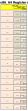
\includegraphics{../../02_Registers/images/X86_64-GP-registers.png}

\end{center}

\end{document} 